\documentclass[template.tex]{subfiles}

\usepackage{comment} 

\begin{document}

\begin{comment}
Andrew's comments: (THIS IS METHODS)
- describe modelling framework and details how you built everything
- now explain in detail what the package is \& can do, what the structure is like
- clarify that it is situated in complexity between custom scripts and modelling tools with graphical interfaces. It would be possible to design a graphical interface for this later on, but that is not the target audience.


"Python is a high-level programming language well suited to rapid development and prototyping, as well as being more accessible to domain scientists than low-level languages such as FORTRAN or C++." - Mobius GMD paper
- This is also due to the dynamic interpretation of python, which makes python slower, but python is rapidly developing and leveraging other lower level language for speed. Also has high functionality for parallelisation of code execution which is very relevant to complex marine ecosystem models. 

- clearly state limitations (scope) of phydra 
- mention that xarray-simlab is general enough to support IBMs! But not developed here.
\end{comment}

 %% \ SECTION 2
\section{The Phydra package: structure \& features} \label{Section:phydrapackage}
% 2nd Section:
% Background, theoretical framework. Specifics here!




The Phydra package is an open-source project embedded within the Python scientific ecosystem. T  

are central to Phydra's function and will be presented below.

The library of modular processes and the user interface are built on functionality borrowed from the Xarray-simlab package \citep{Bovy2018Xarray-simlab:Interactively}. Xarray-simlab provides an object-oriented framework for building and running flexible models within the labelled multi-dimensional data structure of Xarray. The structure stores the variables defined at model setup with their respective labels for easy plotting and postproccesing. Xarrays are easily converted to Netcdf files, the commonly used file format for biogeochemical data. The defined models can take any form, from sequential Games-of-life to large landscape erosion models in the fastscape package \citep{benoit_bovy_2020_3840917}. Xarray-simlab currently only provides step-wise calculation of Python functions acting on defined variables and is not optimised for solving systems of differential equations. 
We use the Python GEKKO Optimisation suite to provide a more robust integration of models built in Phydra,. GEKKO is an open-source, object-oriented library of model construction, analysis and optimisation tools \citep{Beal2018GEKKOSuite}. Models can be constructed based on a common syntax and are compiled to efficient FORTAN code before solving.
Utilizing GEKKO as a back end solver within the Xarray-simlab framework, we keep the benefits of , a native data structure that is natively labelled and documented and the efficient compuation of lower level languages.

Automatic differentiation provides the necessary gradients, accurate to machine precision, without extra work from the user.

that allows more efficient computation of larger models, a modular mathematical syntax from which to build our model,
and a powerful framework for model optimisation.

The GEKKO package 

"GEKKO is an object-oriented Python library that offers model construction, analysis tools, and visualisation of simulation and optimisation."

Both of these Python packages are relatively young and actively being developed, which provides some challenges but also allows for constant improvements to the functionality that Phydra provides.

Below we will describe how Phydra leverages these open-source projects to provide a tool-set to construct, modify, solve, analyse and share marine ecosystem models. In the following sub-sections, the basic modular components of Phydra are discussed and a general model development workflow is presented.






\subsection{Xarray-Simlab: object-oriented modelling framework}
%!
\textit{For now this subsection just includes my bullet points, Benoît Bovy has promised to write it.}
%!

A key point is in the name, xarray-simlab builds a flexible model structure on top xarray -> for labelled multidimensional datasets in python.

This means models in xarray-simlab natively use xarray as the basis for the data structure. A model with the proper parameterisation creates an xarray-dataset, which stores the output after model is run.

This 

- Further detail on the xarray-simlab framework used for phydra!

"xarray-simlab is a Python library that provides both a generic framework for building computational models in a modular fashion and a xarray extension for setting and running simulations using the xarray.Dataset structure. It is designed for fast, interactive and exploratory modelling."

"xarray-simlab is a tool for fast model development and easy, interactive model exploration. It aims at empowering scientists to do better research in less time, collaborate efficiently and make new discoveries."

specific version used here: v0.4.1 \cite{benoit_bovy_2020_3755979}


The xarray-simlab framework is built on a very few concepts that allow great flexibility in model customisation:

- models
- processes
- variables

\subsubsection{Models, processes and variables}
in xarray-simlab, (almost) everything is a process.
- in the following sections, introduce the specific implementation of xarray-simlab processes within phydra, what is actually implemented in v1 and how it can be modified and used.

models

processes

Just describe this in text...!

variables
- foreign variables
- group variables
- on-demand variables
- index variables
- object variables


\subsection{GEKKO Optimization suite: compiled solver back end}

"The GEKKO Python package solves large-scale mixed-integer and differential algebraic equations with nonlinear programming solvers. Modes of operation include machine learning, data reconciliation, real-time optimization, dynamic simulation, and nonlinear model predictive control." \cite{Beal2018GekkoSuite}

"GEKKO is not only an algebraic modeling language (AML) for posing optimization problems in simple object-oriented equation-based models to interface with powerful built-in optimization solvers but is also a package with the built-in ability to run model predictive control, dynamic parameter estimation, real-time optimization, and parameter update for dynamic models on real-time applications. The"

"Algebraic modeling languages (AML) facilitate the interface between advanced solvers and
human users. High-end, off-the-shelf gradient-based solvers require extensive information about the problem, including variable bounds, constraint functions and bounds, objective functions, and first and second derivatives of the functions, all in consistent array format. AMLs simplify the process by allowing the model to be written in a simple, intuitive format."

"GEKKO fills the role of a typical AML, but extends its capabilities to specialize in dynamic
optimization applications. As an AML, GEKKO provides a user-friendly, object-oriented Python interface to develop models and optimization solutions. Python is a free and open-source language that is flexible, popular, and powerful. IEEE Spectrum ranked Python the #1 programming language in 2017. Being a Python package allows GEKKO to easily interact with other popular scientific and numerical packages. Further, this enables GEKKO to connect to any real system that can be accessed through Python. Since Python is designed for readability and ease rather than speed, the Python GEKKO model is
converted to a low-level representation in the Fortran back-end for speed in function calls. Automatic differentiation provides the necessary gradients, accurate to machine precision, without extra work from the user. GEKKO then interacts with the built-in open-source, commercial, and custom large-scale solvers for linear, quadratic, nonlinear, and mixed integer programming (LP, QP, NLP, MILP, and MINLP) in the back-end. Optimization results are loaded back to Python for easy access and further analysis or manipulation."

specific version used here: v0.2.7

\subsubsection{Gekko variable types}
there are more, Gekko is much more complex than our use case, but the ones used in this implementation are
- Parameters. 
- Intermediates. 
- State Variables.  
- Equations.
additionally some functions like summing of terms (sum(x)) or calculating the Euler exponent (exp(x)) have specific implementations that are part of the Gekko library.


\subsection{Phydra: flexible marine ecosystem modelling}

Phydra leverages the objects and syntax provided by Xarray-simlab and GEKKO, to create flexible marine ecosystem models that can be solved efficiently. The GEKKO model instance that handles solving and optimisation is initialised in a Xarray-simlab process and shared between all the processes that constitute a model instance. These processes are object classes that are provided with Phydra. We separate the processes into multiple logical categories that represent logical structures in a marine ecosystem model: Environments, Forcings, Components and Fluxes.

\subsubsection{Environments} \label{Section:PhysicalEnvironment}

A Phydra Environment defines the structure of the ecosystem and provides external inputs (i.e. forcings) that can be accessed by all processes linked to this environment. As a simple example we could take a chemostat model. The flow-through culture system is defined by a solution of nutrients that flows into a tank of fixed volume. Organisms within the tank grow, consume nutrients and are also flushed out of the system with the outflow of the medium. The Environment process in Phydra describing a chemostat would have the nutrient concentration in the flowing substrate, as well as the flow-rate of the system as required external forcing processes. The forcing input can be supplied from different Forcing processes, for example with a time-varying flow rate. Components, which define the state variables in our model, are grouped within our chemostat Environment and the Fluxes (e.g. nutrient uptake or mortality) affect Components within this Environment. We can add any number of Components from the Phydra library into our Environment and between the Components we could add any number of interactions.

Phydra as of now provides an easily modifiable base Environment and implementations of a chemostat Environment, as well as a slab-ocean Environment. The first release of Phydra supports only single zero-dimensional implementations of these basic ecosystem models, but the development of multi-dimensional Environments is a high priority for further development.

\subsubsection{Model forcing (and verification) data} \label{Section:ForcingSection}

To simplify models of complex systems larger processes are not mechanistically implemented, but instead empirically represented as an external forcing. Model forcings and data used in model optimisation are represented by GEKKO parameters that are supplied to the model discretised at the same time-step that the model is solved.

Included with this version of Phydra we have the necessary forcing types that have to be supplied to the provided Environments. For a chemostat model, this is a source concentration of a component in the medium, as well as a flow rate of the system. The slab-ocean Environment interfaces with forcings describing the concentration of a component below the mixed layer, movement of the mixed layer depth (MLD), irradiance at surface and temperature within the mixed layer. There are basic methods supplied to create either constant forcing or values over time based on mathematical functions. Additionally a base Forcing process can be modified by a user to provide any external data, which can then be used by other processes in the library. The flexible class-based structure allows a process class inheriting from the base MLD forcing process to be recognised as an MLD forcing in the Fluxes and processes of our model.

\subsubsection{Components}

An ecosystem model tracks chemical compounds as well as organisms via state variables. These state variables can define completely different species, but can also be multiple state variables within a group that share common processes. Components within Phydra are defined at this higher level and can contain a single state variable or a group of state variables that share a common process.

What is the info defined with a Component:
- Units!
- Name & label within model
- dimensionality! (for now just groups of SV in 0D)

PFT models -> complexity.. this whole issue

- Components are state variables, make sure to use clear wording and explain well

\subsubsection{Fluxes}
Due to the flexible nature of Environments and Components, the interactions between fluxes are dependent 

what is a flux:
- closure or input terms - one component affected
- Any transfer between Components

- Flows are parts of differential equations, that affect one or more components, and can be influenced by forcing and the physical environment


\subsubsection{Installing and running Phydra}
The Phydra package is available via the Python pip package manager, but we encourage using Conda as a package manager that is provided with the scientific Anaconda Python distribution.
Please follow the up-to-date instructions on the Github repository for installation of Phydra and its dependencies.
% CONDA NAME DROP
Since python is a fast developing language, we will provide instructions to install a fully compatible virtual environment with the Conda package manager separate from a users normal python environment. For interactive coding and rapid prototyping we recommend using the Jupyter environment that is available via Conda. For more complex and larger model runs on servers or clusters python scripts are preferable.

\subsection{Model development workflow}

Constructing marine ecosystem models in Phydra is by nature flexible, but the user can follow a general workflow of assembling models from the library of processes. This wokflow is visualized in \ref{Figure:phydraschematics} and will be further explained below.

\subsubsection{Model construction}
Here 
- Dimensionality is a very important fact of building models, and xarray-simlab provides a simple, but sometimes tricky interface for managing dimensionality, so make sure to explain it relatively well here, as well as the implementations.
- I can cite https://www.biogeosciences.net/17/609/2020/ to explain why dimensionality is an important consideration in phytoplankton models.

\subsubsection{Runtime}
- explain what the options are to run the model, depends on if a time implicit method will be added to solve, or if it will just remain with the time explicit steps of xarray-simlab

\subsubsection{Model Diagnostics}
- this is a relevant section, *if* Benoît can help me with creating the ODE visualisation & model diagnostics.

\subsubsection{Parameter fitting}
- this is a relevant section, if i manage to get some decent parameter fitting results for the example 1 and 3.. either only 3 or both, is my feeling. 


\subsubsection{Modification and further development}

- Similar to how a forcing process can easily be subclassed to supply a different forcing, other processes in xsimlab can be easily subclassed and modified to have a different function, as long as the interaction between state variables matches
- Explain interface to process subclasses, and how it is relatively easy to set up xsimlab processes with slightly different  formulations, but the same basic interaction

% OPEN SOURCE CONTRIBUTION 
Phydra (like Xarray-simlab and GEKKO) is an open-source project. Contributions are welcome and in fact greatly appreciated. You can contribute in many ways by reporting bugs, submitting feedback, contributing to the development of the code or the documentation for example. Please read the contributing guidelines on the Github repository for further details.





%%% TWO-COLUMN FIGURES
%
%%f
\begin{figure*}[t]
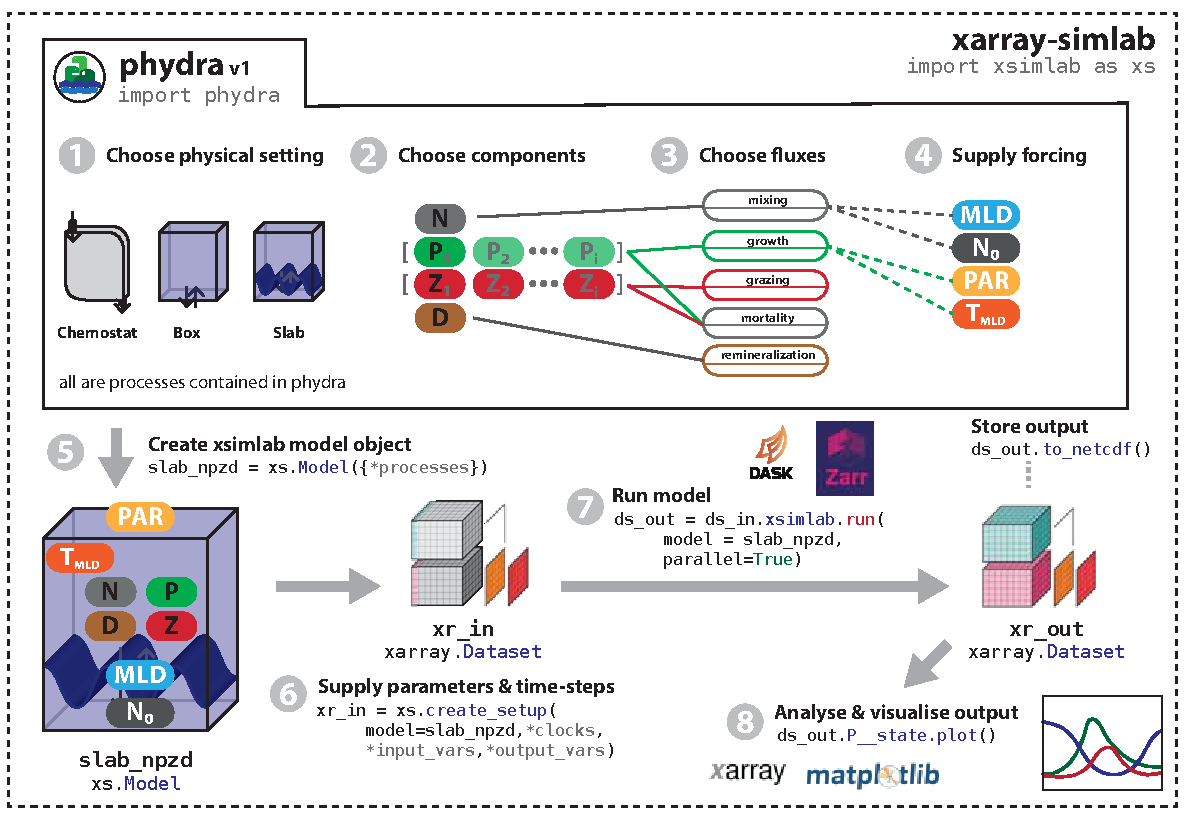
\includegraphics[width=12cm]{Figures/firstdraft_schematics/01__schematics_phydra_1.pdf}
\caption{The phydra package is embedded within the xarray-simlab framework. phydra contains a library of physical settings (1), components (i.e. state variables) (2), fluxes (3) and forcing variables (4), that can be combined and reused to create an xarray-simlab model instance. Xarray-simlab provides the functionality to define the model (5) from processes in the phydra library, supply parameters and create an xarray input (6), then run the model (7) and the resulting output is dynamically stored in another xarray, with fully labelled dimensions and containing all parameters.}
\label{Figure:phydraschematics}
\end{figure*}

general explanation, and then go into detail below (see Figure \ref{Figure:phydraschematics})





% Everything below here is optional, it depends on what I can actually do in the package
% this is a custom function to be able to see references when rendering subfiles:
\biblio

\end{document}